\documentclass{article} % For LaTeX2e
\usepackage{iclr2021_conference,times}
\usepackage{booktabs}
\usepackage{graphicx}
\usepackage{subcaption}
\usepackage{caption}
\usepackage{listings}
\usepackage[colorlinks=true, linkcolor=black, citecolor=black]{hyperref}
\lstset{ 
  language=Python, 
  frame=single, 
  breaklines=true, 
  basicstyle=\small\ttfamily, 
  keywordstyle=\color{blue}, 
  commentstyle=\color{green!40!black},
  stringstyle=\color{red}, 
}


% Optional math commands from https://github.com/goodfeli/dlbook_notation.
\input{math_commands.tex}

\usepackage{hyperref}
\usepackage{url}


\title{Topic 3: Modelling of Real-life MIP Problems}
\iclrfinalcopy%
% Authors must not appear in the submitted version. They should be hidden
% as long as the \iclrfinalcopy macro remains commented out below.
% Non-anonymous submissions will be rejected without review.

\author{The Ikunbelievable Group\thanks{ The Ikunbelievable Group consists of four people who contributed equally to this work:
\begin{tabular}{@{}l}
  Xiaotian Ji (\texttt{Xiaotian.Ji20@student.xjtlu.edu.cn}), \\
  Qiuyi Chen (\texttt{Qiuyi.Chen2002@student.xjtlu.edu.cn}), \\
  Liyuan Jin (\texttt{Liyuan.Jin20@student.xjtlu.edu.cn}),   \\
  Chi Qin (\texttt{Chi.Qin20@student.xjtlu.edu.cn}).%
\end{tabular}%
}
}

% The \author macro works with any number of authors. There are two commands
% used to separate the names and addresses of multiple authors: \And and \AND.
%
% Using \And between authors leaves it to \LaTeX{} to determine where to break
% the lines. Using \AND forces a linebreak at that point. So, if \LaTeX{}
% puts 3 of 4 authors names on the first line, and the last on the second
% line, try using \AND instead of \And before the third author name.

\newcommand{\fix}{\marginpar{FIX}}
\newcommand{\new}{\marginpar{NEW}}

%\iclrfinalcopy % Uncomment for camera-ready version, but NOT for submission.
\begin{document}


\maketitle
\clearpage


\tableofcontents
\clearpage
\section{Introduction}

Lily has recently been accepted by the London School of Economics
and Political Science, majored in Operational Research and her boyfriend,
David, is set to begin his studies at Imperial College London. Eager to make
the most of their summer vacation in Europe before the start of the school
term, they decide to embark on a memorable 2-week trip, exploring famous
European cities.

David, a music enthusiast, wants to visit Vienna, and Lily is keen on the Van
Gogh Museum in Amsterdam. Considering their interests, they choose nine
destinations: Vienna, Paris, Rome, Barcelona, Berlin, Amsterdam, Copenhagen,
Zurich, and Budapest. They prefer traveling by train and plane, but due to
Lily's past witness of a tragic plane crash, they will limit their plane trips.

To plan their itinerary, they must organize their routes considering time,
cost, and visiting all desired destinations while accounting for varying train
and plane ticket prices. Unsure of where to start, they seek assistance from
the Ikunbelievable Group.

\section{Problem Description}

\subsection{Input and Objective}

\begin{enumerate}
  \item Cities: For their graduation trip, they have chosen 10 representative cities,
        including London, Vienna, Paris, Barcelona, Berlin, Amsterdam, Copenhagen
        (København), Zurich, and Budapest.
  \item Transportation Options: They will consider to take plane or train to travel
        between these cities.
  \item Time: We will consider the time required to travel between cities by plane and
        train.
  \item Price: Since ticket prices can vary from month to month, in early May, we
        calculated the average price of tickets from July 1 to July 14, from 8 AM to 8 PM.\@
  \item Customization: To account for individual preferences, we will input different
        weights for cost and time, allowing each traveler to prioritize factors that
        are most important to them when selecting the optimal travel itinerary.
\end{enumerate}

Their objective is to find the optimal travel route under the assumptions and
the constraints described below.

\subsection{Assumptions}

We make the following assumptions to develop a comprehensive travel plan that
caters to different individual preferences.

\begin{enumerate}
  \item The travel time and cost between city A and city B are identical in both
        directions.
  \item Two modes of transportation, train and plane, are considered, despite the
        existence of alternative choices.
  \item The trip must begin and end in a specific city, in Lily and David's case,
        London, as they need to store their luggage at the school in London and take
        only essential items for the journey.
  \item Considering factors like public health events and peak travel seasons, we
        averaged ticket prices between July 1st and 14th, from
        8 AM to 8 PM, to determine ticket prices and minimize the impact of outliers.
\end{enumerate}

\subsection{Constraints}

Our goal is to identify the best transportation options for various groups with
diverse needs, enabling efficient travel across all cities. Therefore, some
constraints are as followed:

\begin{enumerate}
  \item Each city can only be visited once.
  \item We set maximum limits for plane and train usage because some individuals may
        have constraints on taking planes or trains due to personal preferences,
        coupons for free food, or memberships with airlines or train companies
        providing extra luxury services.
\end{enumerate}

\subsection{Toy Example}

Now we demonstrate a simple example to show the consequence of implementing
different traveling routes.

\subsubsection{Toy Example's Input}
\begin{itemize}
  \item Cities: For the trip in the summer vocation, traveling from Anhui Province to
        Guangdong Province, choose 3 representative cities, including Guangzhou,
        Shenzhen, and Foshan.
  \item Transportation Options: Only consider to take plane or train to travel between
        these cities.
  \item Time: Only consider the time required to travel between cities by plane and
        train.
  \item Price: The fares used were based on real prices observed around one month in
        advance, in June 2022.
  \item Customization: Only consider the total cost, and don't care about the time.
\end{itemize}

\subsubsection{Toy Example's Assumptions}
\begin{itemize}
  \item The travel time and cost between city A and city B are identical in both
        directions.
  \item The trip starts and ends in Hefei.
\end{itemize}

\subsubsection{Toy Example's Constraints}
\begin{itemize}
  \item Each city can only be visited once.
  \item No limit to the number of times for taking trains and planes.
\end{itemize}

The ticket prices and travel routes are displayed with black lines representing airplane routes and blue lines indicating train routes. In Figure~\ref{fig:Optimalchoice}, the optimal choice is priced at ¥1200. Figure~\ref{fig:Higherprice} presents an alternative option that costs ¥1645, resulting in an increased expenditure of approximately ¥450.
\begin{figure}[!ht]
  \centering
  \begin{subfigure}{0.3\textwidth}
    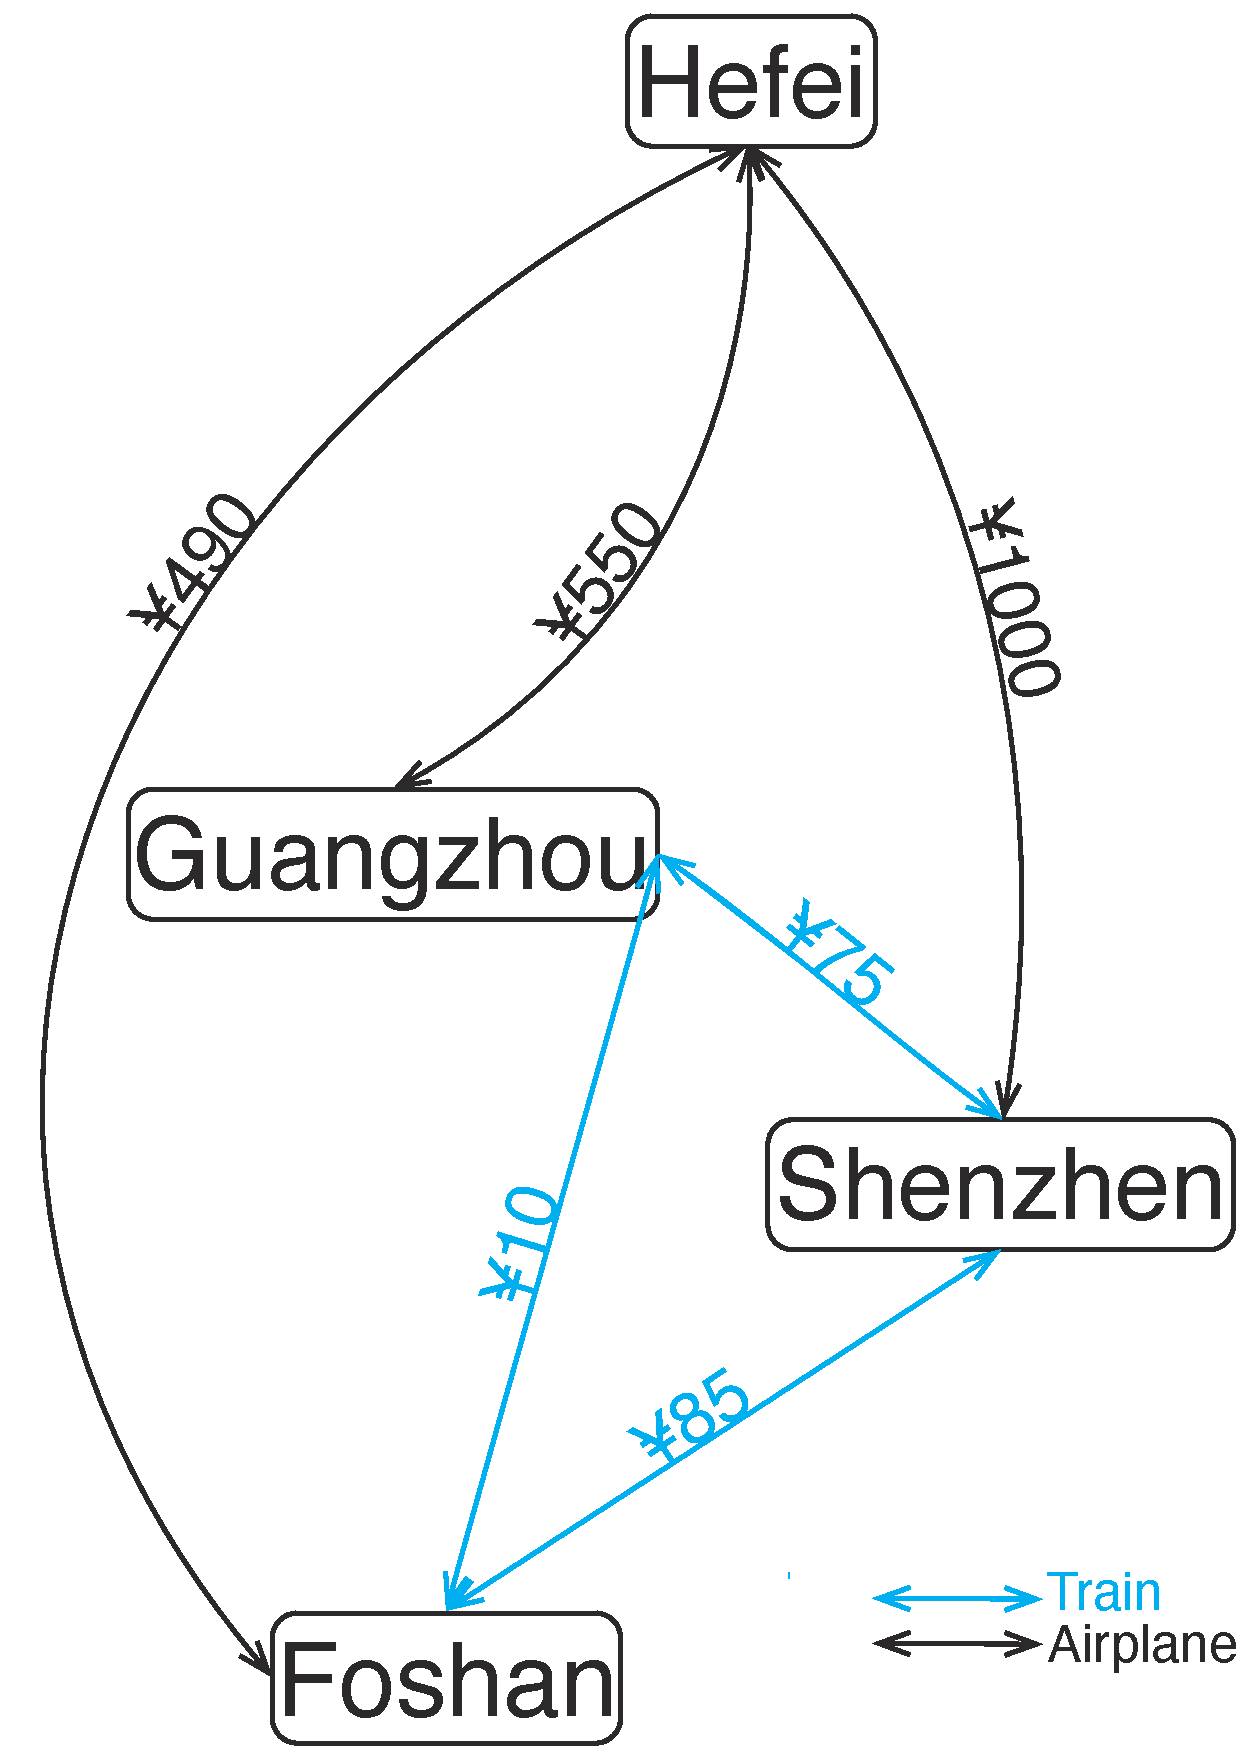
\includegraphics[width=0.85\textwidth]{/Users/badudu/Documents/MTH203/CW2/report/pic/toy_all.jpg}
    \caption{Ticket Prices}%
    \label{fig:Ticketprice}
  \end{subfigure}
  \hfill % Add space between images
  \begin{subfigure}{0.3\textwidth}
    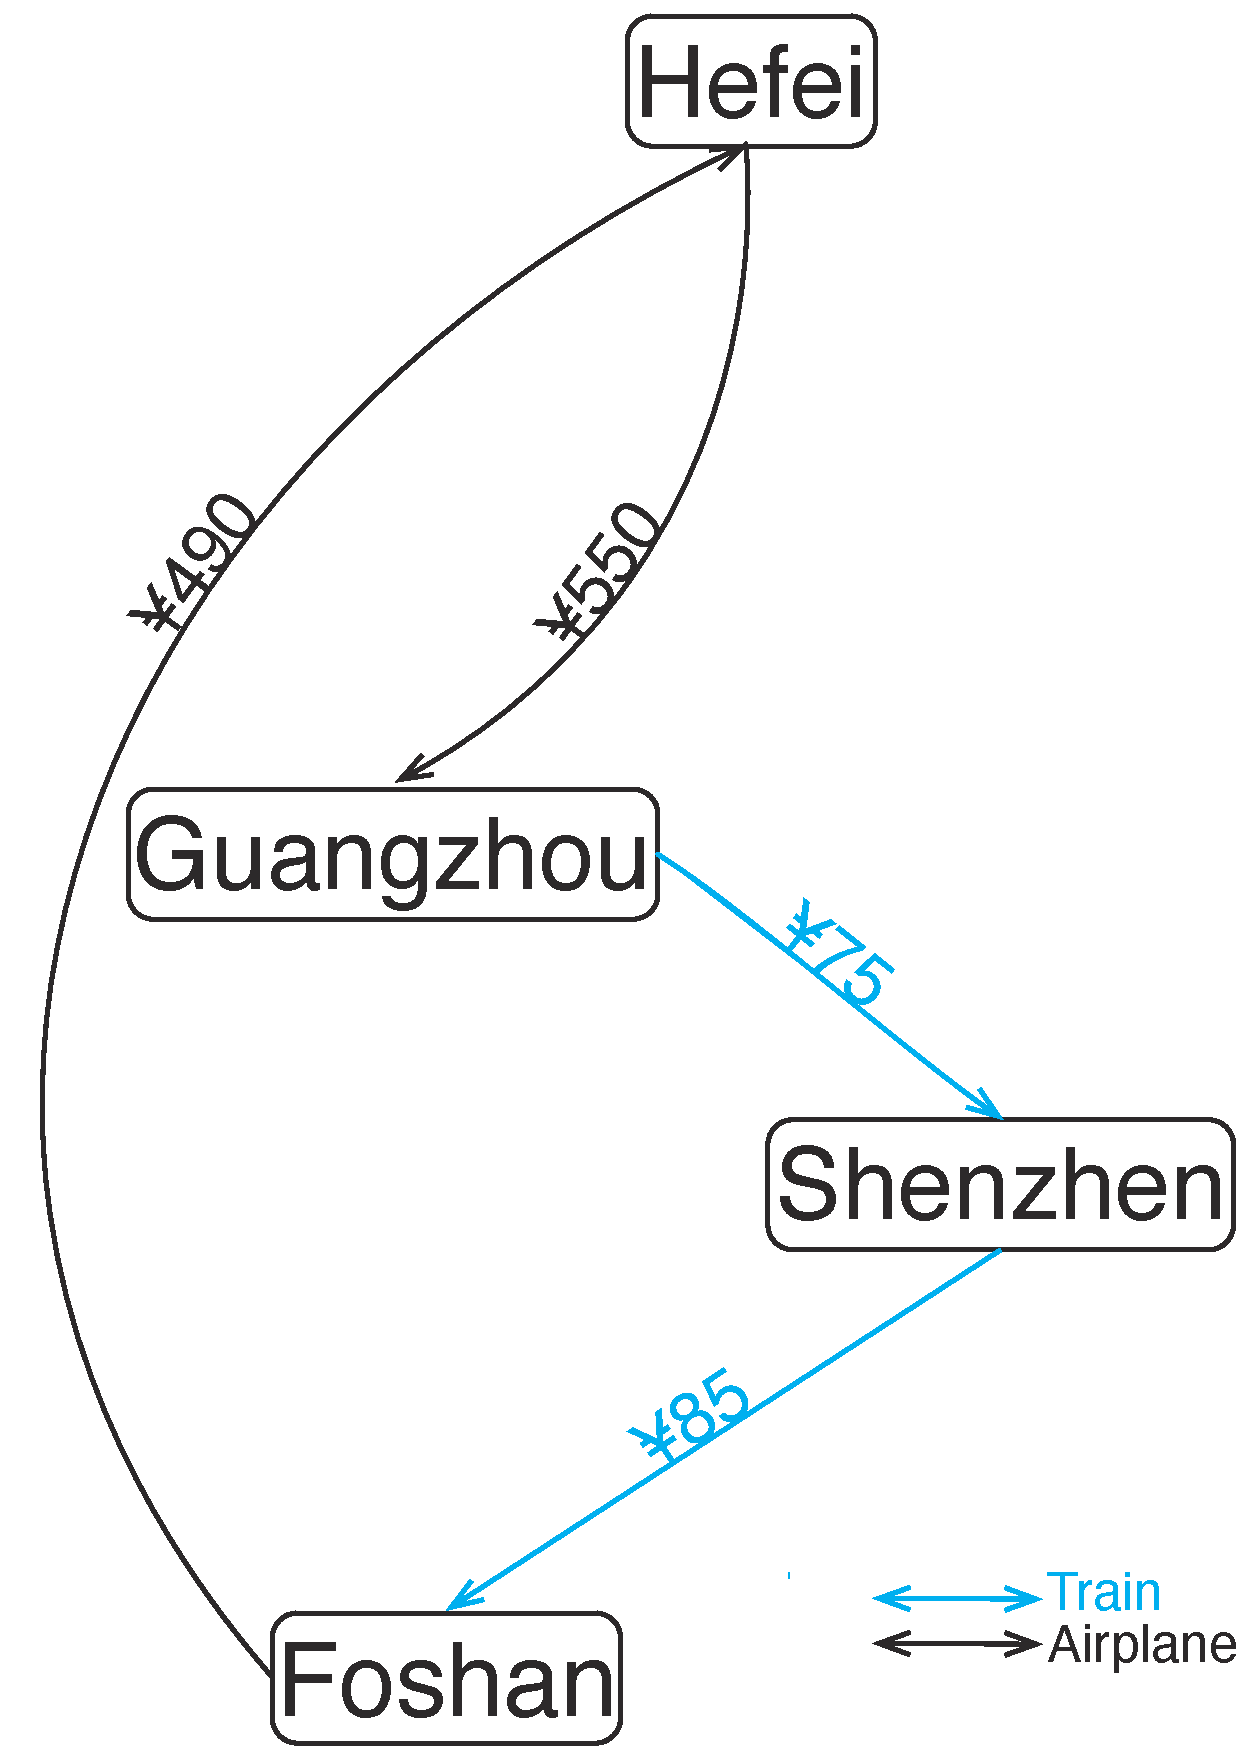
\includegraphics[width=0.85\textwidth]{/Users/badudu/Documents/MTH203/CW2/report/pic/optimal.jpg}
    \caption{Optimal Choice}%
    \label{fig:Optimalchoice}
  \end{subfigure}%
  \hfill % Add space between images
  \begin{subfigure}{0.3\textwidth}
    \includegraphics[width=0.85\textwidth]{/Users/badudu/Documents/MTH203/CW2/report/pic/higher_price.jpg}
    \caption{Choice With Higher Price}%
    \label{fig:Higherprice}
  \end{subfigure}%
  \caption{Toy Example}
\end{figure}
\clearpage
\section{MIP Model}
Let $G_1(V_1, E_1)$ and $G_2(V_2, E_2)$ be two given graphs, each with their
respective vertex and edge sets. Define a positive edge weight function $w :
  E_1 \cup E_2 \rightarrow \mathbb{R}^+$. We construct a new graph $G(V, E)$,
where $V = V_1 \cup V_2$ and $E = E_1 \cup E_2$. The objective is to find a
Hamiltonian cycle in $G$ that minimizes the objective function. In order to
achieve this, we introduce binary variables $x_{ij}^k$ for edge selection from
either $G_1$ or $G_2$.

Formally, let $x_{ij}^k \in \{0, 1\}$ be a binary variable such that:

\begin{equation*}
  x_{ij}^k =
  \begin{cases}
    1, & \text{if edge } (i, j) \text{ from graph } G_k \text{ is selected,} \\
    0, & \text{otherwise.}
  \end{cases}
\end{equation*}

The goal is to determine the values of $x_{ij}^k$ that lead to a Hamiltonian
cycle with the minimum objective function value in the graph $G$. It can be
written as:
\begin{equation*}
  \text{minimize} \, f = \sum_{k=1}^{2} \sum_{(i,j) \in E_k} w_{ij}^k x_{ij}^k
\end{equation*}

Subject to the following \textbf{constraints}:

\begin{enumerate}
  \item Each vertex has a total degree of 2, with one incoming edge (in-degree) and one
        outgoing edge (out-degree) from either graph $G_1$ or $G_2$.

        \begin{equation*}
          \sum_{k=1}^{2} \sum_{j \in V} x_{ij}^k = 2, \quad \forall i \in V
        \end{equation*}
  \item No subtours are allowed (subtour elimination constraint):

        \begin{equation}
          \sum_{(i,j) \in S \times (V \setminus S)} x_{ij}^k \geq 2, \quad \forall S \subset V, S \neq \emptyset, S \neq V, k \in \{1, 2\}\label{eq:Nosubtour}
        \end{equation}

        Here, $S$ is a subset of $V$, and $(V \setminus S)$ is the complement of $S$ in
        $V$.\eqref{eq:Nosubtour} ensures that there are no smaller cycles within the
        Hamiltonian cycle.
  \item The number of edges selected from $G_1$ and $G_2$ are no more than $N_1$ and
        $N_2$ respectively.

        \begin{equation*}
          \sum_{(i,j) \in E_1} x_{ij}^1 \leq N_1 \quad \text{and} \quad \sum_{(i,j) \in E_2} x_{ij}^2 \leq N_2,  \quad \forall i,j \in V
        \end{equation*}
\end{enumerate}

\subsection*{Variables and Parameters}
\begin{itemize}
  \item $G_1(V_1, E_1)$ and $G_2(V_2, E_2)$ store the information of airplane's and train's transportation modes.
  \item The vertices $V_1$ and $V_2$ in each graph represent cities in different
        countries.
  \item $k$ is an index representing the transportation mode in the given graphs. Specifically, $k = 1$ corresponds to the airplane transportation mode in graph $G_1$, and $k = 2$ corresponds to the train transportation mode in graph $G_2$.
  \item If there is an edge between the vertices, it indicates that travel between the
        cities is accessible using either mode of transportation. We can represent an
        edge between vertex $i$ and $j$ as $(i, j) \in E_k$, where $k \in \{1, 2\}$.
  \item The edges store $cost$ and $time$, which represent the one-way ticket price and
        travel time, respectively. So the weight function $w$ is defined as:
        \begin{equation*}
          w_{ij}^k = \alpha \cdot \text{cost}_{ij}^k + \beta \cdot \text{time}_{ij}^k, \quad where \quad \alpha + \beta = 1
        \end{equation*}
        where $\alpha$ and $\beta$ are the weights of the cost and time attributes
        respectively.

\end{itemize}
Therefore, our objective function can be further written as:

\begin{equation*}
  \text{minimize}\, f = \sum_{k=1}^{2} \sum_{(i,j) \in E_k} (\alpha \cdot \text{cost}_{ij}^k + \beta \cdot \text{time}_{ij}^k) x_{ij}^k
\end{equation*}

\section{Computational Results}
%todo appendix
To find how different constraints and weight functions influence the consequence, we write a Python solver with held-kalp (``See \citet{doi:10.1137/0110015} for more information'') and the raw data and code are shown in the~\ref{para:appendix}ppenix. 

After evaluating unconstrained air and train travel options, we present three recommendations based on varying cost and time priorities. Our objective function f incorporates $\alpha$ and $\beta$ as weights. In~Table~\ref{tab:alpha1beta0} ($\alpha = 1, \beta = 0$) highlights the least expensive route, while~Table~\ref{tab:alpha0beta1} ($\alpha = 0, \beta = 1$) showcases the quickest option. Table~\ref{tab:alpha0.3beta0.7} ($\alpha = 0.3, \beta = 0.7$) offers a balanced choice, taking only 20 minutes longer than the fastest plan but saving 1,300 yuan, making it a potentially superior option after extensive iterations.

\begin{table}[!ht]
  \centering
  \begin{tabular}{llrrr}
    \toprule
    Segment                          & Transportation Mode & Cost (¥) & Time (hours) \\
    \midrule
    London $\rightarrow$  Barcelona  & Airplane            & 532.0    & 2.5          \\
    Barcelona $\rightarrow$  Paris   & Airplane            & 590.0    & 2.0          \\
    Paris $\rightarrow$  Rome        & Airplane            & 292.0    & 2.25         \\
    Rome $\rightarrow$  Vienna       & Airplane            & 344.0    & 1.45         \\
    Vienna $\rightarrow$  Budapest   & Train               & 175.0    & 2.63         \\
    Budapest $\rightarrow$  Berlin   & Train               & 420.0    & 14.0         \\
    Berlin $\rightarrow$  Copenhagen & Train               & 240.0    & 5.0          \\
    Copenhagen $\rightarrow$  Amsterdam & Train            & 469.0    & 16.0         \\
    Amsterdam $\rightarrow$  Zurich  & Train               & 525.0    & 10.0         \\
    Zurich $\rightarrow$  London     & Airplane            & 616.0    & 1.83         \\
    \midrule
    Total                            &                     & 4203.0   & 57.66         \\
    \bottomrule
  \end{tabular}
  \caption{$\alpha=1, \beta=0, N_1=N_2=10$}%
  \label{tab:alpha1beta0}
\end{table}


\begin{table}[!ht]
  \centering
  \begin{tabular}{llrrr}
    \toprule
    Segment                          & Transportation Mode & Cost (¥) & Time (hours) \\
    \midrule
    London $\rightarrow$  Paris      & Airplane            & 459.0    & 1.05         \\
    Paris $\rightarrow$  Budapest    & Airplane            & 1171.0   & 0.83         \\
    Budapest $\rightarrow$  Vienna   & Airplane            & 794.0    & 0.83         \\
    Vienna $\rightarrow$  Rome       & Airplane            & 344.0    & 1.45         \\
    Rome $\rightarrow$  Barcelona    & Airplane            & 634.0    & 2.0          \\
    Barcelona $\rightarrow$  Zurich  & Airplane            & 760.0    & 1.92         \\
    Zurich $\rightarrow$  Copenhagen & Airplane            & 855.0    & 1.75         \\
    Copenhagen $\rightarrow$  Berlin & Airplane            & 317.0    & 1.0          \\
    Berlin $\rightarrow$  Amsterdam  & Airplane            & 967.0    & 1.4          \\
    Amsterdam $\rightarrow$  London  & Airplane            & 940.0    & 1.1          \\
    \midrule
    Total                            &                     & 7241.0   & 13.33        \\
    \bottomrule
  \end{tabular}
  \caption{$\alpha=0, \beta=1, N_1=N_2=10$}%
  \label{tab:alpha0beta1}
\end{table}

\begin{table}[!ht]
  \centering
  \begin{tabular}{llrrr}
    \toprule
    Segment                          & Transportation Mode & Cost (¥) & Time (hours) \\
    \midrule
    London $\rightarrow$  Paris      & Airplane            & 459.0    & 1.05         \\
    Paris $\rightarrow$  Zurich      & Airplane            & 608.0    & 1.3          \\
    Zurich $\rightarrow$  Barcelona  & Airplane            & 760.0    & 1.92         \\
    Barcelona $\rightarrow$  Rome    & Airplane            & 634.0    & 2.0          \\
    Rome $\rightarrow$  Vienna       & Airplane            & 344.0    & 1.45         \\
    Vienna $\rightarrow$  Budapest   & Airplane            & 794.0    & 0.83         \\
    Budapest $\rightarrow$  Berlin   & Airplane            & 537.0    & 1.5          \\
    Berlin $\rightarrow$  Copenhagen & Airplane            & 317.0    & 1.0          \\
    Copenhagen $\rightarrow$  Amsterdam & Airplane          & 559.0    & 1.5          \\
    Amsterdam $\rightarrow$  London  & Airplane            & 940.0    & 1.1          \\
    \midrule
    Total                            &                     & 5952.0   & 13.65        \\
    \bottomrule
  \end{tabular}
  \caption{$\alpha=0.3, \beta=0.7, N_1=N_2=10$}%
  \label{tab:alpha0.3beta0.7}
\end{table}

Since Lily has witnessed a plane crash, she hopes to limit the air travels within N times. However, none of the former results fits Lily's constraint of flight number. If we limit the flights within 5 times, the calculation shows that no matter what alpha is, the optimal route remains the same, which is shown in~Table~\ref{tab:alpha0.3beta0.7N14} when $N_1=4, N_2=10$. 

\begin{table}[!ht]
  \centering
  \begin{tabular}{llrrr}
    \toprule
    Segment                          & Transportation Mode & Cost (¥) & Time (hours) \\
    \midrule
    London $\rightarrow$  Copenhagen & Airplane            & 669.0    & 2.0          \\
    Copenhagen $\rightarrow$  Barcelona & Airplane          & 1214.0   & 3.0          \\
    Barcelona $\rightarrow$  Rome     & Airplane            & 634.0    & 2.0          \\
    Rome $\rightarrow$  Budapest     & Airplane            & 489.0    & 1.67         \\
    Budapest $\rightarrow$  Vienna    & Train               & 175.0    & 2.63         \\
    Vienna $\rightarrow$  Zurich      & Train               & 630.0    & 8.0          \\
    Zurich $\rightarrow$  Berlin      & Train               & 455.0    & 9.0          \\
    Berlin $\rightarrow$  Amsterdam   & Train               & 599.0    & 6.3          \\
    Amsterdam $\rightarrow$  Paris    & Train               & 697.0    & 3.5          \\
    Paris $\rightarrow$  London       & Train               & 1148.0   & 2.0          \\
    \midrule
    Total                            &                     & 6710.0   & 40.3         \\
    \bottomrule
  \end{tabular}
  \caption{$\alpha=0.3, \beta=0.7, N_1=4, N_2=10$}%
  \label{tab:alpha0.3beta0.7N14}
\end{table}


According to the calculation above, we recommend Lily to limit their times of flight into 6 times and consider $\alpha = 0.7, \beta = 0.3$ to meet the balance between cost and time, along with the fear for taking the plane.

\section{Conclusion}
We have presented an approach to find an optimal travel route for Lily and David, considering different transportation modes: airplanes and trains. We have formulated the problem as a Graph Structural Mixed Integer Problem, where nodes and edges represent information about the two transportation modes. A binary variable, $x$, is used to control whether a particular mode of transportation is chosen or not. We defined an objective function based on weighted costs and times to optimize the overall travel experience.

We analyzed various scenarios, giving different weights to cost and time attributes, as well as considering the constraint of limiting the number of flights due to Lily's fear of flying. Computational results show that when the number of flights is limited to 6 and the weight of cost is 0.7, while the weight of time is 0.3, we achieve a balanced travel plan that accommodates Lily's concerns and still provides a satisfactory travel experience for the group.

The research presented here can be extended in the future. As the complexity of the optimization algorithm itself is an NP-hard problem, the time required for the solver to find a solution may increase exponentially when the number of cities is too large. Therefore, optimizing the algorithm or finding local optimal solutions offers room for improvement. Moreover, measuring the concept of cost-effectiveness remains vague and is only derived from our observations after thousands of experiments. The difficulty in defining cost-effectiveness lies in its subjective nature, as it varies from person to person. However, our results are helpful to Lily and her friends, and we wish them a great time on their journey.

\bibliography{iclr2021_conference}
\bibliographystyle{iclr2021_conference}

\clearpage
\appendix
\section{Appendix}%
\label{para:appendix}
% This is the raw data for ticket price in Table~\ref{tab:airplane} and Table~\ref{tab:train}.

\begin{table}[!ht]
  \centering
  \begin{tabular}{lllllllllll}

     & London & Vienna & Paris & Rome & Barcelona & Berlin & Amsterdam & København & Zurich & Budapest \\

  London & 0 & 545 & 459 & 769 & 532 & 559 & 940 & 669 & 616 & 296 \\

  Vienna & 545 & 0 & 868 & 344 & 742 & 880 & 1367 & 931 & 3456 & 794 \\

  Paris & 459 & 868 & 0 & 292 & 590 & 635 & 921 & 718 & 608 & 1171 \\

  Rome & 769 & 344 & 292 & 0 & 634 & 820 & 1819 & 1109 & 690 & 489 \\
  Barcelona & 532 & 742 & 590 & 634 & 0 & 840 & 1104 & 1214 & 760 & 728 \\
  Berlin & 559 & 880 & 635 & 820 & 840 & 0 & 967 & 317 & N/A & 537 \\
  Amsterdam & 940 & 1367 & 921 & 1819 & 1104 & 967 & 0 & 559 & 1049 & 1269 \\
  København & 669 & 931 & 718 & 1109 & 1214 & 317 & 559 & 0 & 855 & 613 \\
  Zurich & 616 & 3456 & 608 & 690 & 760 & N/A & 1049 & 855 & 0 & 2650 \\
  Budapest & 296 & 794 & 1171 & 489 & 728 & 537 & 1269 & 613 & 2650 & 0 \\
  \end{tabular}
  \caption{Travel cost (¥) of Airplane between cities in July}%
  \label{tab:costairplane}
\end{table}

\begin{table}[!ht]
  \centering
  \begin{tabular}{lllllllllll}

     & London & Vienna & Paris & Rome & Barcelona & Berlin & Amsterdam & København & Zurich & Budapest \\

  London & 0 & 1351 & 1148 & N/A & 2541 & 1015 & 753 & 1680 & 1155 & 3150 \\

  Vienna & 1351 & 0 & 1072 & 365 & 1778 & 625 & 552 & 565 & 630 & 175 \\

  Paris & 1148 & 1072 & 0 & 770 & 1386 & 691 & 697 & 1078 & 1120 & 980 \\

  Rome & N/A & 365 & 770 & 0 & N/A & 1036 & 974 & N/A & 840 & 1750 \\

  Barcelona & 2541 & 1778 & 1386 & N/A & 0 & 2249 & 2073 & 2940 & 2450 & 4060 \\

  Berlin & 1015 & 625 & 691 & 1036 & 2249 & 0 & 599 & 240 & 455 & 420 \\

  Amsterdam & 753 & 552 & 697 & 974 & 2073 & 599 & 0 & 469 & 525 & 595 \\

  København & 1680 & 565 & 1078 & N/A & 2940 & 240 & 469 & 0 & 2002 & 665 \\

  Zurich & 1155 & 630 & 1120 & 840 & 2450 & 455 & 525 & 2002 & 0 & 1050 \\

  Budapest & 3150 & 175 & 980 & 1750 & 4060 & 420 & 595 & 665 & 1050 & 0 \\
  \end{tabular}
  \caption{Travel cost (¥) of Train between cities in July}%
  \label{tab:costtrain}
\end{table}

\begin{table}[!ht]
  \centering
  \begin{tabular}{lllllllllll}

     & London & Vienna & Paris & Rome & Barcelona & Berlin & Amsterdam & København & Zurich & Budapest \\

  London & 0 & 2.25 & 1.05 & 2.6 & 2.5 & 2 & 1.1 & 2 & 1.83 & 2.67 \\

  Vienna & 2.25 & 0 & 2 & 1.45 & 2.5 & 1.1 & 1.8 & 1.5 & 1.3 & 0.83 \\

  Paris & 1.05 & 2 & 0 & 2.25 & 2 & 1.8 & 1.3 & 2 & 1.3 & 0.83 \\

  Rome & 2.6 & 1.45 & 2.25 & 0 & 2 & 2 & 2.25 & 2.5 & 1.58 & 1.67 \\

  Barcelona & 2.5 & 2.5 & 2 & 2 & 0 & 2.55 & 2.3 & 3 & 1.92 & 2.67 \\

  Berlin & 2 & 1.1 & 1.8 & 2 & 2.55 & 0 & 1.4 & 1.5 & N/A & 1.5 \\

  Amsterdam & 1.1 & 1.8 & 1.3 & 2.25 & 2.3 & 1.4 & 0 & 1.67 & 1.75 & 2.08 \\

  København & 2 & 1.5 & 2 & 2.5 & 3 & 1 & 1.5 & 0 & N/A & 2 \\

  Zurich & 1.83 & 1.3 & 1.3 & 1.58 & 1.92 & N/A & 1.67 & N/A & 0 & 1.67 \\

  Budapest & 2.67 & 0.83 & 0.83 & 1.67 & 2.67 & 1.5 & 2.08 & 2 & 1.67 & 0 \\
  \end{tabular}
  \caption{Travel time (in hours) of Airplane between cities in July}%
  \label{tab:timeairplane}
\end{table}

\begin{table}[!ht]
  \centering
  \begin{tabular}{lllllllllll}

     & London & Vienna & Paris & Rome & Barcelona & Berlin & Amsterdam & København & Zurich & Budapest \\

  London & 0 & 14 & 2 & N/A & 11 & 11 & 3.9 & 27 & 8 & 24 \\

  Vienna & 14 & 0 & 11 & 17.5 & 35 & 12 & 14 & 17.6 & 8 & 2.63 \\

  Paris & 2 & 11 & 0 & 10.5 & 6.75 & 8.8 & 3.5 & 14.5 & 4.5 & 13.42 \\

  Rome & N/A & 17.5 & 10.5 & 0 & N/A & 25 & 32 & N/A & 8 & 27 \\

  Barcelona & 11 & 35 & 6.75 & N/A & 0 & 23.3 & 20 & 35 & 15 & 32 \\

  Berlin & 11 & 12 & 8.8 & 25 & 23.3 & 0 & 6.3 & 5 & 9 & 14 \\

  Amsterdam & 3.9 & 14 & 3.5 & 32 & 20 & 6.3 & 0 & 16 & 10 & 21 \\

  København & 27 & 17.6 & 14.5 & N/A & 35 & 5 & 16 & 0 & 18.4 & 21 \\

  Zurich & 8 & 8 & 4.5 & 8 & 15 & 9 & 10 & 18.4 & 0 & 11 \\

  Budapest & 24 & 2.63 & 13.42 & 27 & 32 & 14 & 21 & 21 & 11 & 0 \\
  \end{tabular}
  \caption{Travel time (in hours) of Train between cities in July}%
  \label{tab:timetrain}
\end{table}
\clearpage
The solver script is also available on \url{https://github.com/Beautifuldog01/CW2/tree/main}
\begin{lstlisting}
import itertools
import pandas as pd
import numpy as np
from tqdm import tqdm
import os
import csv


def read_and_process_csv(file_name):
    matrix = []

    with open(file_name, 'r') as file:
        reader = csv.reader(file)
        for row in reader:
            new_row = [np.nan if cell == '' else float(cell) for cell in row]
            matrix.append(new_row)

    matrix = np.array(matrix, dtype=float)
    n = matrix.shape[0]
    matrix[np.isnan(matrix)] = 0

    for i in range(n):
        for j in range(i + 1, n):
            matrix[i, j] = matrix[j, i]

    # matrix_nonzero = matrix[matrix > 0]
    # matrix_min = np.min(matrix_nonzero)
    # matrix_max = np.max(matrix_nonzero)
    # matrix[matrix > 0] = (matrix[matrix > 0] - matrix_min) / (matrix_max - matrix_min)

    matrix[matrix == 0] = 1000

    return matrix


def combined_cost_and_transport(path, flight_df, train_df, max_flights, max_trains):
    total_cost = 0
    transport = []
    flight_count = 0
    train_count = 0
    for i in range(len(path) - 1):
        flight_cost = flight_df.loc[path[i], path[i + 1]]
        train_cost = train_df.loc[path[i], path[i + 1]]
        if flight_count < max_flights and (train_count >= max_trains or flight_cost < train_cost):
            total_cost += flight_cost
            transport.append("Airplane")
            flight_count += 1
        elif train_count < max_trains:
            total_cost += train_cost
            transport.append("Train")
            train_count += 1
        else:
            return float('inf'), transport
    return total_cost, transport


def tsp_bruteforce_combined(flight_data, train_data, start, max_flights, max_trains):
    cities = flight_data.columns.tolist()
    cities.remove(start)
    min_cost = float('inf')
    min_path = None
    min_transport = None
    for path in tqdm(list(itertools.permutations(cities)), desc="Calculating progress"):
        path = (start,) + path + (start,)
        cost, transport = combined_cost_and_transport(path, flight_data, train_data, max_flights, max_trains)
        if cost < min_cost:
            min_cost = cost
            min_path = path
            min_transport = transport

    return min_path, min_cost, min_transport


cities = ['London', 'Vienna', 'Paris', 'Rome', 'Barcelona', 'Berlin', 'Amsterdam', 'Copenhagen', 'Zurich', 'Budapest']


def read_month_data(directory):
    data = {}
    for file_name in os.listdir(directory):
        if file_name.endswith(".csv"):
            data_type = file_name[:-4]
            file_path = os.path.join(directory, file_name)
            data[data_type] = read_and_process_csv(file_path)
    return data


july_data_path = "/Users/badudu/Documents/MTH203/CW2/code/data/July"
august_data_path = "/Users/badudu/Documents/MTH203/CW2/code/data/August"

july_data = read_month_data(july_data_path)
# august_data = read_month_data(august_data_path)

flight_cost_df = pd.DataFrame(july_data['flight_costs'], columns=cities, index=cities)
train_cost_df = pd.DataFrame(july_data['train_costs'], columns=cities, index=cities)
flight_time_df = pd.DataFrame(july_data['flight_time'], columns=cities, index=cities)
train_time_df = pd.DataFrame(july_data['train_time'], columns=cities, index=cities)


def read_original_data(file_name):
    data = []

    with open(file_name, 'r') as file:
        reader = csv.reader(file)
        for row in reader:
            new_row = [np.nan if cell == '' else float(cell) for cell in row]
            data.append(new_row)

    data_df = pd.DataFrame(data, columns=cities, index=cities)

    n = data_df.shape[0]
    for i in range(n):
        for j in range(i + 1, n):
            data_df.iloc[i, j] = data_df.iloc[j, i]

    return data_df


flight_cost_original_df = read_original_data(os.path.join(july_data_path, 'flight_costs.csv'))
train_cost_original_df = read_original_data(os.path.join(july_data_path, 'train_costs.csv'))
flight_time_original_df = read_original_data(os.path.join(july_data_path, 'flight_time.csv'))
train_time_original_df = read_original_data(os.path.join(july_data_path, 'train_time.csv'))


def get_cost_and_time(optimal_path, optimal_transport, flight_cost_matrix, train_cost_matrix, flight_time_matrix,
                      train_time_matrix):
    cost_list = []
    time_list = []

    for i in range(len(optimal_path) - 1):
        city1 = optimal_path[i]
        city2 = optimal_path[i + 1]
        transport = optimal_transport[i]

        if transport == "Airplane":
            cost = flight_cost_matrix.loc[city1, city2]
            time = flight_time_matrix.loc[city1, city2]
        else:  # transport == "Train"
            cost = train_cost_matrix.loc[city1, city2]
            time = train_time_matrix.loc[city1, city2]

        cost_list.append(cost)
        time_list.append(time)

    return cost_list, time_list


from functools import lru_cache


def held_karp_modified(flight_df, train_df, start_city, max_flights, max_trains):
    cities = flight_df.columns.tolist()
    cities.remove(start_city)
    cities_set = frozenset(cities)

    @lru_cache(maxsize=None)
    def dp(city, visited_cities, remaining_flights, remaining_trains):
        if visited_cities == cities_set:
            if remaining_flights > 0:
                return flight_df.loc[city, start_city], [start_city]
            else:
                return train_df.loc[city, start_city], [start_city]

        min_cost = float('inf')
        min_path = []

        for next_city in cities:
            if next_city not in visited_cities:
                new_visited_cities = visited_cities | {next_city}
                flight_cost = flight_df.loc[city, next_city]
                train_cost = train_df.loc[city, next_city]

                if remaining_flights > 0:
                    cost_flight, path_flight = dp(next_city, new_visited_cities, remaining_flights - 1,
                                                  remaining_trains)
                    cost_flight += flight_cost

                    if cost_flight < min_cost:
                        min_cost = cost_flight
                        min_path = path_flight + [next_city]

                if remaining_trains > 0:
                    cost_train, path_train = dp(next_city, new_visited_cities, remaining_flights, remaining_trains - 1)
                    cost_train += train_cost

                    if cost_train < min_cost:
                        min_cost = cost_train
                        min_path = path_train + [next_city]

        return min_cost, min_path

    min_cost, optimal_path = dp(start_city, frozenset(), max_flights, max_trains)
    optimal_path = [start_city] + optimal_path[::-1]

    # Determine transport mode
    transport = []
    for i in range(len(optimal_path) - 1):
        if max_flights > 0 and (flight_df.loc[optimal_path[i], optimal_path[i + 1]] <= train_df.loc[
            optimal_path[i], optimal_path[i + 1]] or max_trains == 0):
            transport.append("Airplane")
            max_flights -= 1
        else:
            transport.append("Train")
            max_trains -= 1

    return optimal_path, min_cost, transport


alpha = 0.35
beta = 1 - alpha
optimal_li = []
flight_df = flight_cost_df * alpha + flight_time_df * beta * 500
train_df = train_cost_df * alpha + train_time_df * beta * 500
start_city = cities[0]
max_flights = 10
max_trains = 10
optimal_path, min_cost, optimal_transport = tsp_bruteforce_combined(flight_df, train_df, start_city, max_flights,
                                                                    max_trains)
cost_list, time_list = get_cost_and_time(optimal_path, optimal_transport, flight_cost_original_df,
                                         train_cost_original_df, flight_time_original_df, train_time_original_df)
optimal_li.append([optimal_path, optimal_transport, sum(cost_list), sum(time_list)])
print("Optimal path:", optimal_path)
print("Transportation mode:", optimal_transport)
print("Costs for each segment:", cost_list)
print("Times for each segment:", time_list)
  \end{lstlisting}
\end{document}
